\chapter{Shape-space Models and B-Spline Curves}
\label{chapter:bspline}
In the CCD algorithms, a parametric curve model is responsible for
restricting Region of Interest (ROI) and providing prior knowledge. 
Throughout this thesis, visual curves are represented in terms of
parametric spline curves which is widely applied in computer graphics.

In this chapter, we introduce a deformable 2-D model called
shape-space models.  In the first section, we start by explaining
spline functions and their construction. Details on how parametric
curves are constructed from spline functions are discussed in the
later section. This forms the basis for the CCD approach.
\section{B-Spline Function}
\label{sec:bsc}
In mathematics, every spline function of a given degree,
smoothness, and domain partition, can be represented as a linear
combination of B-splines of that same degree and smoothness, and over
that same partition~\cite{press2007numerical}. In terms of this statement, we can
construct  a spline curve parametrized by spline functions that are
expressed as linear combinations of B-splines. 

Given a non-decreasing vector of real values $U = [u_0, \ldots,
u_{m-1}]$ called knot vector, with $u_i$ called the knot, a
B-spline of degree n is a parametric curve
\begin{equation}
  \label{eq:4.1}
  \mathbf{C}(u) =  \sum_{i=0}^{m-n-2} P_{i} B_{i,n}(u) \mbox{ , } u \in [u_{n},u_{m-n-1}]
\end{equation}

where $P_i$ are called control points, $B_{i,n}$ are called
basic function. For n=0,1,...,m-2, the m-n-1 basis B-splines of degree
n can be defined as 

\begin{eqnarray}
  \label{eq:4.2}
  B_{i,0}(u) &=&  \left\{
\begin{matrix} 
1 & \mathrm{if} \quad u_i \leq u < u_{i+1} \\
0 & \mathrm{otherwise} 
\end{matrix}
\right.,\qquad i=0,\ldots, m{-}2 \nonumber\\
B_{i,n}(u) &=& \frac{u - u_i}{u_{i+n} - u_i} B_{i,n-1}(u) + \frac{u_{i+n+1} - u}{u_{i+n+1} - u_{i+1}} B_{i+1,n-1}(u)
, i=0,\ldots, m{-}n{-}2.  
\end{eqnarray}

Furthermore, we can write the B-spline compactly in matrix notation as 
\begin{equation}
  \label{eq:4.3}
  \mathbf{C}(u) = 
  \begin{pmatrix}
\mathbf{B}(u)^T & 0 \\
0 &\mathbf{B}(u)^T
  \end{pmatrix}
\mathbf{P}
\end{equation}

where vector $\mathbf{P}$ denotes the axis components of control
points
\begin{equation}
  \label{eq:4.4}
  \mathbf{P} =
  \begin{pmatrix}
    P_x & P_y    
  \end{pmatrix}^T \quad \mathrm{where} \quad P_x =
  \begin{pmatrix}
    P_0^x\\
    \cdots\\
    \cdots\\
    P_{N-1}^x
  \end{pmatrix}
\end{equation}
Where $N$ denotes the number of control points. $\mathbf{B}(u)$ is a
vector of basis function
\begin{equation}
  \label{eq:4.5}
  \mathbf{B}(u) = (B_0(u), \ldots, B_{N-1}(u))^T
\end{equation}

A example of B-spline curve for different basic functions is depicted
in Fig.~\ref{fig:bspline}. The B-spline is said to be uniform when the knots are equidistant,
otherwise non-uniform. In this thesis, for simplicity, we only
consider the uniform case.
\begin{figure}[htb]
  \centering
  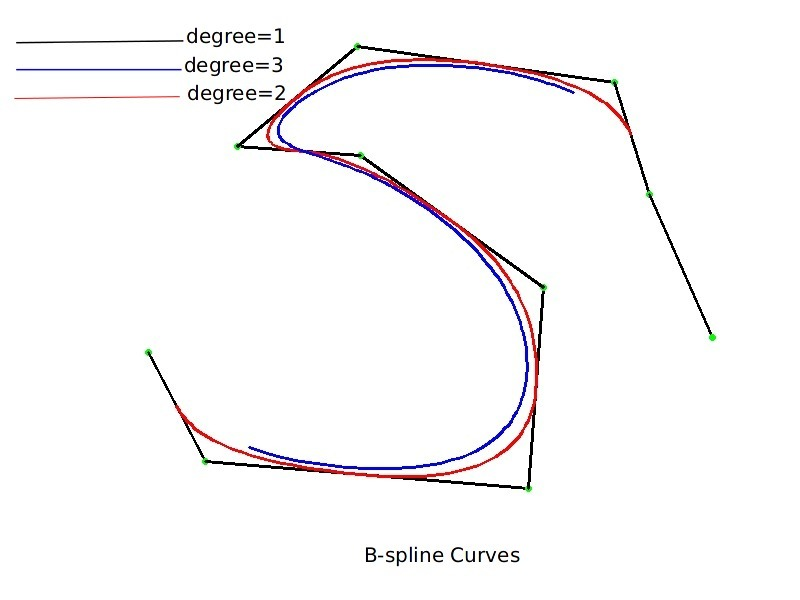
\includegraphics[width=10cm]{images/bspline.jpg}
  \caption[B-spline curves for different degrees~\cite{contourpanin2011}]{Red, green and black
    curves respectively represent the one for degree 1,2 and 3.}
\label{fig:bspline}
\end{figure}

As two special examples of the B-Spline, we consider the matrix form and
derivative of uniform quadratic and cubic B-Spline respectively.

\subsection{Uniform quadratic B-Spline}
\label{sec:uqb}

Because the knot-vector is equidistant, the blending function can
easily be computed. In each segment, the blending function shares the
same form, as following
\begin{equation}
  \label{eq:4.3}
  \mathbf{b}_{i,2}(u) = \begin{cases} \frac{1}{2}u^2 \\ -u^2 + u + \frac{1}{2} \\ \frac{1}{2}(1-u)^2   \end{cases}
\end{equation}

Its derivative is 
\begin{equation}
  \label{eq:4.4}
  \mathbf{b}_{i,2}'(u) = \begin{cases} u \\ -2u + 1 \\ u-1   \end{cases}
\end{equation}

The matrix-form of uniform quadratic B-Spline is given by
\begin{equation}
  \label{eq:4.5}
\mathbf{B}_i(u) = \begin{bmatrix} u^2 & u & 1 \end{bmatrix} \frac{1}{2} \begin{bmatrix}
1 & -2 & 1 \\
-2 &  2 & 0 \\
1 &  1 & 0 \end{bmatrix}
\end{equation}.

\subsection{Uniform cubic B-Spline}
\label{sec:uqb}
Uniform cubic B-Spline is the most commonly used form of B-Spline, 
the blending function is
\begin{equation}
  \label{eq:4.6}
  \mathbf{b}_{i,3}(u) = \begin{cases} \frac{1}{6}(-u^3+3u^2-3u+1) \\
    \frac{1}{6}(3u^3 -6u^2+4)\\ \frac{1}{6}(-3u^3+3u^2+3u+1) \\
    \frac{1}{6}u^3
   \end{cases}
\end{equation}

Its derivative can be written as
\begin{equation}
  \label{eq:4.7}
  \mathbf{b}_{i,3}'(u) = \begin{cases} \frac{1}{2}(-u^2+2u-1) \\
    \frac{1}{2}(3u^2 -4u)\\ \frac{1}{2}(-3u^2+2u+1) \\
    \frac{1}{2}u^2
   \end{cases}
\end{equation}


Its matrix-form is given by
\begin{equation}
  \label{eq:4.8}
\mathbf{B}_i(u) = \begin{bmatrix} u^3 & u^2 & u & 1 \end{bmatrix} \frac{1}{6} \begin{bmatrix}
-1 &  3 & -3 & 1 \\
 3 & -6 &  3 & 0 \\
-3 &  0 &  3 & 0 \\
 1 &  4 &  1 & 0 \end{bmatrix}
\begin{bmatrix} \mathbf{p}_{i-1} \\ \mathbf{p}_{i} \\ \mathbf{p}_{i+1} \\ \mathbf{p}_{i+2} \end{bmatrix}
\end{equation}.

\section{Parametric B-spline curve}
\label{sec:pbc}

In a 2-D image, a curve is composed of many discrete points which are
identified by their coordinates. For those points on a curve, their axis
components $x$, $y$ are particular functions of knots value $u$, known
as splines. Hence, we can define a B-spline curve as 
\begin{equation}
  \label{eq:4.11}
  \mathbf{C}(u) = (x(u),y(u))^T = \mathbf{U}(u) \mathbf{P}
\end{equation}
where $\mathbf{U}(u)$ denotes the matrix mapping control point vector P to image
curve $\mathbf{C}(u)$
\begin{equation}
  \label{eq:4.12}
  \mathbf{U}(u) =   \begin{pmatrix}
\mathbf{B}(u)^T & 0 \\
0 &\mathbf{B}(u)^T
  \end{pmatrix}
\end{equation}.

\subsection{Norm for B-spline curves}
\label{sec:nbc}

Norm and inner product of curves are useful in curve approximation. In
an image plan, using the Euclidean distance measure, we can define the
norm for curves as 
\begin{equation}
  \label{eq:4.13}
  \left| \left| \mathbf{C} \right|\right|^2  = \mathbf{C}^T\mathcal{U}\mathbf{C}
\end{equation}

where $\mathcal{U}$ represents the metric matrix for curves, and can be
defined as 
\begin{equation}
  \label{eq:4.14}
  \mathcal{U} =   \begin{pmatrix}
\mathcal{B}^T & 0 \\
0 &\mathcal{B}^T
  \end{pmatrix}  
\end{equation}

$\mathcal{B}$ denotes the metric matrix for a given class of B-spline
function
\begin{equation}
  \label{eq:4.15}
  \mathcal{B}   = \frac{1}{L} \int_0^L \mathbf{B}(u)\mathbf{B}(u)^T \mathrm{d}u
\end{equation}

In Fig.~\ref{fig:bsplinenormal}, we use B-spline to sketch the contour of a
cola bottle.
\begin{figure}[htb]
  \centering
  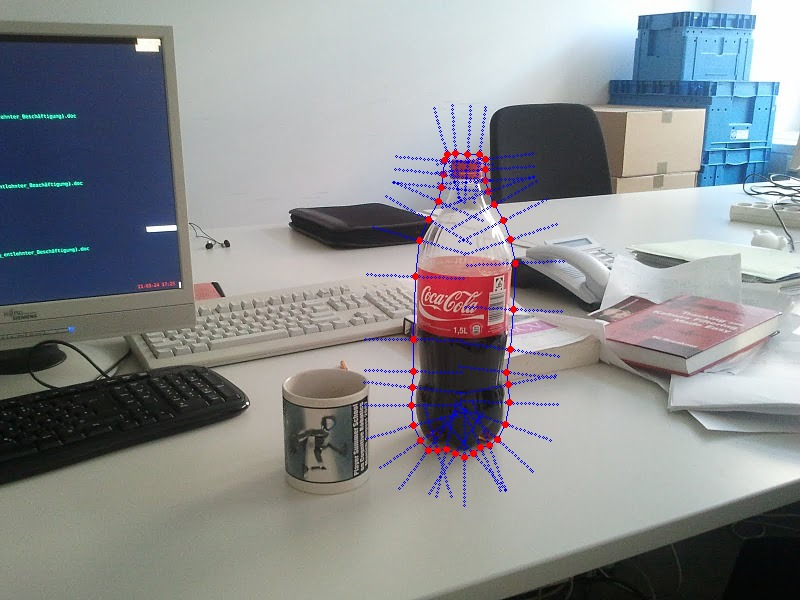
\includegraphics[width=10cm]{images/bsplinenormal.jpg}
  \caption{The contour of a bottle is sketched using a B-spline
    curve, the blue points are pixels on the perpendicular of the contour.}
\label{fig:bspline}
\end{figure}


\section{Shape-space models}
\label{sec:ssm}

The shape-space $\mathcal{S}$ is a linear parameterisation of the set of allowed
deformations of a base curve(AC). From the perspective of mathematics, shape-space
$\mathcal{S} = \mathcal{S}(\mathbf{A},\mathbf{P})$ is a linear mapping of a shape-space
vector $\mathbf{\Phi} \in  \mathbb{R}^{N_{\mathbf{\Phi}}}$ to a spline vector $\mathbf{C} \in
\mathbb{R}^{Np}$:
\begin{equation}
  \label{eq:4.16}
  \mathbf{C} = \mathbf{A}\mathbf{X}+ \mathbf{P}
\end{equation}

where $T$ is a $Np \times N_{\mathbf{\Phi}}$ shape-matrix. The
constant  $P_0$ is a deformable template curve. (AC), Usually, the
dimension $N_{\mathbf{\Phi}}$ of the shape-space vector is clearly
smaller than the dimension of the spline-vector $Np$. This makes the
problem more simple and computationally cheaper.

In this chapter, we consider a important shape space named planar
affine. The planar affine has 6 degree of freedom: horizontal
translation, vertical translation, rotation, horizontal scale,
vertical scale and diagonal scale. The planar affine group can be
viewed as the class of all linear transformations that can be applied
to a template curve $\mathbf{C}$(AC). 

\begin{equation}
  \label{eq:4.17}
  \mathbf{C(u)} = \mathbf{T} + \mathbf{M} \mathbf{C}_0(u)
\end{equation}

where $T = (T_1, T_2)^T$ represents the two-dimensional translation
vector, and $M$ is a $2 \times 2$ matrix to control the rotation and
scaling, so that $T$ and $M$ together can represent the 6 degree of
freedom of planar Affine space. We can write the shape-matrix $\mathbf{A}$
as 
\begin{equation}
  \label{eq:4.18}
  A =
  \begin{bmatrix}
    1 & 0 & P_0^x & 0 & 0 & P_0^y\\
    0 & 1 & 0 & P_0^y & P_0^x & 0
  \end{bmatrix}
\end{equation}

The model parameters can be interpreted as
\begin{equation}
  \label{eq:4.19}
  \mathbf{\Phi} =  (T_1, T_2, M_{11} - 1, M_{22} - 1, M_{21}, M_{12})
\end{equation}

The planar affine shape-space discussed above can be extended for
three-dimensional affine shape-space, which is more suitable for a
non-planar object. The new space-model needs 8 degrees of  freedom to
make up of the six-parameter planar affine space and a two-parameter
extension. The transformation matrix for the three-dimensional case
can be written as:

\begin{equation}
  \label{eq:4.20}
  A =
  \begin{bmatrix}
    1 & 0 & P_0^x & 0 & 0 & P_0^y & P_0^z & 0\\
    0 & 1 & 0 & P_0^y & P_0^x & 0 & 0 & 0 & P_0^z
  \end{bmatrix}  
\end{equation}

the three-dimensional affine shape-space components have
the following interpretation:
\begin{equation}
  \label{eq:4.19}
  \mathbf{\Phi} =  (T_1, T_2, M_{11} - 1, M_{22} - 1, M_{21}, M_{12},
  \nu_1, \nu_2)
\end{equation}
where $\nu_1$, $\nu_2$ are the two additional basis elements.








